\index{parallel computing}
\index{distributed computing}
\chapter{Parallel \& Distributed Computing}
\newthought{Scaling Numerical Methods to Massive Problems}


% ==============================================================================================
% INTRODUCTION BLOCK

\section{The Why}
\index{parallel computing!motivation}

\newthought{Throughout this course,} we've assumed computations happen sequentially on a single processor.
But modern AI operates at unprecedented scale:

\begin{table*}[ht]
\centering
\begin{tabular}{p{0.15\textwidth}p{0.20\textwidth}p{0.35\textwidth}}
\toprule
\textbf{Model} & \textbf{Parameters} & \textbf{Training Compute} \\
\midrule
GPT-2 & 1.5B & $\sim 10^{20}$ FLOPS \\
GPT-3 & 175B & $\sim 3.14 \times 10^{23}$ FLOPS \\
GPT-4 & $\sim$1.8T & $\sim 10^{25}$ FLOPS \\
\bottomrule
\end{tabular}
\vspace{2em}
\caption{The scale of modern language models: parameter counts and training compute have grown exponentially.}
\label{tab:model_scale}
\end{table*}

\newthought{A single CPU} performs $\sim 10^{10}$ FLOPS (10 GFLOPS).
Training GPT-3 sequentially would take: $3.14 \times 10^{23} / 10^{10} \approx 10^{13}$ seconds $\approx$ 300,000 years.

\marginnote{\newthought{The solution:} Parallelism. GPT-3 was trained on thousands of GPUs working together. Understanding how this works is essential for modern AI practitioners.}

\newthought{In machine learning and artificial intelligence:}
\begin{itemize}
    \item \textbf{GPUs:} Thousands of cores for parallel matrix operations
    \item \textbf{Data parallelism:} Same model, different data on each GPU
    \item \textbf{Model parallelism:} Split model across devices
    \item \textbf{Distributed training:} Coordinate across multiple machines
\end{itemize}

\newthought{Key insight:} All the numerical methods we've learned---matrix multiplication, gradient computation, convolution---can be parallelized. Understanding parallelism means understanding how modern AI scales.



\newpage
\subsection{Hands On Experience}
\index{parallel computing!hands-on}

\newthought{Consider multiplying} two $1000 \times 1000$ matrices.

\textbf{Sequential:} $2 \times 1000^3 = 2 \times 10^9$ operations.
At 10 GFLOPS: 0.2 seconds.

\textbf{On GPU with 5000 cores:}
Each core handles part of the computation in parallel.
Theoretical speedup: up to 5000$\times$.
Actual speedup: $\sim 100-1000\times$ (limited by memory bandwidth).

\marginnote{\newthought{Why not 5000$\times$?} Memory bandwidth, synchronization overhead, and Amdahl's law limit actual speedup. But the GPU still wins dramatically.}

\newthought{Matrix multiplication is embarrassingly parallel:}
\begin{itemize}
    \item Each output element $C_{ij} = \sum_k A_{ik} B_{kj}$ is independent
    \item Different elements can be computed simultaneously
    \item Perfect fit for GPU architecture
\end{itemize}

This is why neural networks---which are mostly matrix multiplications---benefit so much from GPUs.


\vspace{2.5em}
\newthought{The Learning Objectives} of this chapter aim at providing you with the abilities to:
\begin{itemize}
    \item Understand the scale challenge in modern AI
    \item Distinguish CPU vs. GPU architectures
    \item Apply data parallelism for training neural networks
    \item Understand model parallelism for large models
    \item Synthesize the numerical methods foundation of modern AI
\end{itemize}




% ==============================================================================================
% MAIN THEORY BLOCK - PART A: COMPLEXITY ANALYSIS

\newpage
\section{Complexity Analysis}
\index{Big-O notation}

\subsection{Big-O Notation}

\newthought{Big-O notation} describes how algorithm runtime scales with input size.

\begin{equation}
    f(n) = O(g(n)) \quad \text{means} \quad |f(n)| \leq C \cdot |g(n)| \text{ for large } n
\end{equation}

\marginnote{\newthought{Why Big-O matters:} For $n = 10^6$ data points:
\begin{itemize}
    \item $O(n)$: $10^6$ ops $\approx$ 1 ms
    \item $O(n^2)$: $10^{12}$ ops $\approx$ 15 min
    \item $O(n^3)$: $10^{18}$ ops $\approx$ 30 years
\end{itemize}}

\newthought{Common complexity classes:}

\begin{table*}[ht]
\centering
\begin{tabular}{p{0.2\textwidth}p{0.28\textwidth}p{0.3\textwidth}}
\toprule
\textbf{Notation} & \textbf{Name} & \textbf{Example} \\
\midrule
$O(1)$ & Constant & Array access \\
$O(\log n)$ & Logarithmic & Binary search \\
$O(n)$ & Linear & Single loop \\
$O(n \log n)$ & Linearithmic & Merge sort, FFT \\
$O(n^2)$ & Quadratic & Nested loops \\
$O(n^3)$ & Cubic & Matrix multiplication \\
$O(2^n)$ & Exponential & Brute-force combinatorics \\
\bottomrule
\end{tabular}
\vspace{2em}
\caption{Common complexity classes with examples.}
\label{tab:complexity_classes}
\end{table*}


\begin{figure}[h]
    \centering
    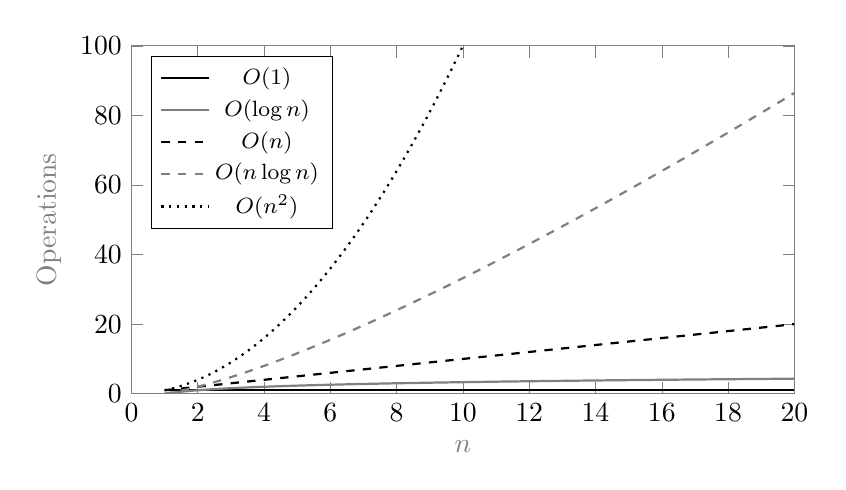
\begin{tikzpicture}
        \begin{axis}[
            width=10cm,
            height=6cm,
            xlabel={$n$},
            ylabel={Operations},
            xmin=0, xmax=20,
            ymin=0, ymax=100,
            tick style={gray},
            label style={gray},
            axis line style={gray},
            legend pos=north west,
            legend style={font=\footnotesize},
        ]
        \addplot[black, thick, domain=1:20, samples=50] {1};
        \addlegendentry{$O(1)$}
        \addplot[gray, thick, domain=1:20, samples=50] {ln(x)/ln(2)};
        \addlegendentry{$O(\log n)$}
        \addplot[black, dashed, thick, domain=1:20, samples=50] {x};
        \addlegendentry{$O(n)$}
        \addplot[gray, dashed, thick, domain=1:20, samples=50] {x*ln(x)/ln(2)};
        \addlegendentry{$O(n \log n)$}
        \addplot[black, dotted, thick, domain=1:10, samples=50] {x^2};
        \addlegendentry{$O(n^2)$}
        \end{axis}
    \end{tikzpicture}
    \caption{Growth rates of common complexity classes. The difference becomes dramatic as $n$ increases.}
    \label{fig:complexity_growth}
\end{figure}



\subsection{Time Complexity of Numerical Methods}
\index{time complexity}

\newthought{Per-iteration costs:}

\begin{table*}[ht]
\centering
\begin{tabular}{p{0.22\textwidth}p{0.28\textwidth}p{0.28\textwidth}}
\toprule
\textbf{Algorithm} & \textbf{Per-Iteration Cost} & \textbf{Notes} \\
\midrule
Grid search & $O(N^d)$ total & Exponential in dimension! \\
Newton 1D & $O(1)$ & Evaluate $f$, $f'$ \\
Secant 1D & $O(1)$ & Evaluate $f$ twice \\
Newton $n$D & $O(n^3)$ & Jacobian inversion \\
Gradient descent & $O(n \cdot p)$ & $n$ samples, $p$ parameters \\
SGD & $O(b \cdot p)$ & $b$ = batch size \\
\bottomrule
\end{tabular}
\vspace{2em}
\caption{Per-iteration costs of common numerical optimization algorithms.}
\label{tab:per_iteration_costs}
\end{table*}

\marginnote{\newthought{The curse of dimensionality:} Grid search with $N = 10$ points per dimension in $d = 100$ dimensions requires $10^{100}$ evaluations---more than atoms in the universe.}

\newthought{Key insight:} SGD replaces $n$ (dataset size) with $b$ (batch size). For ImageNet with $n = 10^6$ and $b = 256$, that's $4000\times$ cheaper per iteration!



\subsection{Convergence Rates}
\index{convergence rate}

\newthought{Convergence rate} describes how fast the error decreases:

\begin{table*}[ht]
\centering
\begin{tabular}{p{0.12\textwidth}p{0.28\textwidth}p{0.16\textwidth}p{0.22\textwidth}}
\toprule
\textbf{Rate} & \textbf{Definition} & \textbf{Example} & \textbf{Meaning} \\
\midrule
Linear & $|e_{k+1}| \leq c \cdot |e_k|$, $c < 1$ & Gradient descent & Error shrinks by constant factor \\
Superlinear & $|e_{k+1}| \leq c \cdot |e_k|^\phi$, $\phi > 1$ & Secant ($\phi \approx 1.618$) & Better than linear \\
Quadratic & $|e_{k+1}| \leq c \cdot |e_k|^2$ & Newton & Digits double each iteration \\
Sublinear & $|e_k| \leq c / k^\alpha$ & SGD on convex & Slow, but $O(1/\sqrt{k})$ \\
\bottomrule
\end{tabular}
\vspace{2em}
\caption{Convergence rates of iterative methods.}
\label{tab:convergence_rates}
\end{table*}

\newthought{Example: Reaching error $\varepsilon = 10^{-12}$ from $e_0 = 1$}

\begin{itemize}
    \item \textbf{Linear} ($c = 0.5$): Need $k$ where $0.5^k < 10^{-12}$, so $k > 40$ iterations
    \item \textbf{Quadratic}: Need $k$ where $e_k < 10^{-12}$
    \begin{itemize}
        \item $e_1 \approx 1$, $e_2 \approx 10^{-1}$, $e_3 \approx 10^{-2}$, $e_4 \approx 10^{-4}$, $e_5 \approx 10^{-8}$, $e_6 \approx 10^{-16}$
        \item Only $\sim 6$ iterations!
    \end{itemize}
\end{itemize}



\subsection{Total Runtime Analysis}
\index{runtime analysis}

\newthought{Total runtime} = iterations $\times$ cost per iteration.

\marginnote{\newthought{The trade-off:} Newton has few iterations but expensive ones. GD has many iterations but cheap ones. Which wins depends on problem size.}

\newthought{Example: Optimizing a quadratic with $n$ parameters}

\begin{table*}[ht]
\centering
\begin{tabular}{p{0.18\textwidth}p{0.2\textwidth}p{0.2\textwidth}p{0.2\textwidth}}
\toprule
\textbf{Method} & \textbf{Iterations} & \textbf{Cost/iter} & \textbf{Total} \\
\midrule
Newton & $\sim 5$ & $O(n^3)$ & $O(5n^3)$ \\
GD & $\sim 1000$ & $O(n)$ & $O(1000n)$ \\
\bottomrule
\end{tabular}
\vspace{2em}
\caption{Total runtime comparison for optimizing a quadratic with $n$ parameters.}
\label{tab:total_runtime}
\end{table*}

\newthought{Break-even:} $5n^3 = 1000n \Rightarrow n^2 = 200 \Rightarrow n \approx 14$.

\begin{itemize}
    \item For $n < 14$: Newton is faster
    \item For $n > 14$: GD is faster
    \item For $n = 10^6$ (typical DNN): GD is $\sim 10^{12}$ times faster!
\end{itemize}



\subsection{Memory Complexity}
\index{memory complexity}

\newthought{Memory matters} as much as time for large problems.

\begin{table*}[ht]
\centering
\begin{tabular}{p{0.18\textwidth}p{0.28\textwidth}p{0.32\textwidth}}
\toprule
\textbf{Method} & \textbf{Memory} & \textbf{For $n = 10^8$} \\
\midrule
Newton & $O(n^2)$ (Hessian) & $10^{16}$ floats $\approx$ 40 PB \\
GD & $O(n)$ (gradient) & $10^8$ floats $\approx$ 400 MB \\
SGD & $O(n)$ (gradient) & $10^8$ floats $\approx$ 400 MB \\
Adam & $O(3n)$ (moments) & $3 \times 10^8$ floats $\approx$ 1.2 GB \\
\bottomrule
\end{tabular}
\vspace{2em}
\caption{Memory complexity of optimization methods.}
\label{tab:memory_complexity}
\end{table*}

\marginnote{\newthought{ResNet-50} has $\sim 25$ million parameters. Its Hessian would have $6.25 \times 10^{14}$ entries, requiring $\sim 2.5$ PB of memory. This is why we use first-order methods.}

\newthought{This is why Newton is impossible for DNNs:} Even storing the Hessian is infeasible.



% ==============================================================================================
% MAIN THEORY BLOCK - PART B

\newpage
\section{The Scale Problem}
\index{scale}

\newthought{Why parallelism is necessary:}

\begin{table*}[ht]
\centering
\begin{tabular}{p{0.30\textwidth}p{0.22\textwidth}p{0.22\textwidth}}
\toprule
\textbf{Task} & \textbf{Sequential Time} & \textbf{With 1000 GPUs} \\
\midrule
Train GPT-3 & 300,000 years & $\sim 1$ month \\
Train ResNet-50 on ImageNet & 2 months & $\sim 1$ hour \\
One forward pass (GPT-3) & 30 seconds & $\sim 100$ ms \\
\bottomrule
\end{tabular}
\vspace{2em}
\caption{Parallelism transforms impossible tasks into routine operations.}
\label{tab:parallelism_speedup}
\end{table*}

\newthought{Types of parallelism:}

\begin{enumerate}
    \item \textbf{Data parallelism:} Same model on different data
    \item \textbf{Model parallelism:} Different parts of model on different devices
    \item \textbf{Pipeline parallelism:} Different layers on different devices
    \item \textbf{Tensor parallelism:} Split individual operations
\end{enumerate}

\begin{figure}[h]
    \centering
    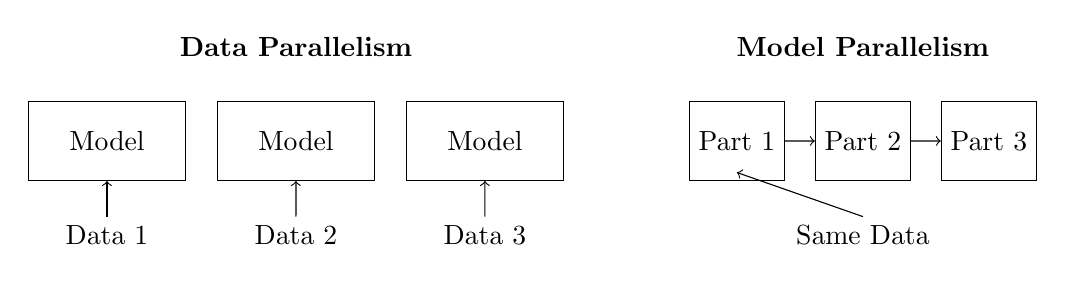
\begin{tikzpicture}[scale=0.8]
        % Data parallelism
        \node[draw, rectangle, minimum width=2cm, minimum height=1cm] (m1) at (0, 2) {Model};
        \node[draw, rectangle, minimum width=2cm, minimum height=1cm] (m2) at (3, 2) {Model};
        \node[draw, rectangle, minimum width=2cm, minimum height=1cm] (m3) at (6, 2) {Model};
        \node at (0, 0.5) {Data 1};
        \node at (3, 0.5) {Data 2};
        \node at (6, 0.5) {Data 3};
        \draw[->] (0, 0.8) -- (m1);
        \draw[->] (3, 0.8) -- (m2);
        \draw[->] (6, 0.8) -- (m3);
        \node at (3, 3.5) {\textbf{Data Parallelism}};

        % Model parallelism
        \node[draw, rectangle, minimum width=1.2cm, minimum height=1cm] (p1) at (10, 2) {Part 1};
        \node[draw, rectangle, minimum width=1.2cm, minimum height=1cm] (p2) at (12, 2) {Part 2};
        \node[draw, rectangle, minimum width=1.2cm, minimum height=1cm] (p3) at (14, 2) {Part 3};
        \draw[->] (p1) -- (p2);
        \draw[->] (p2) -- (p3);
        \node at (12, 0.5) {Same Data};
        \draw[->] (12, 0.8) -- (10, 1.5);
        \node at (12, 3.5) {\textbf{Model Parallelism}};
    \end{tikzpicture}
    \caption{Data parallelism replicates the model; model parallelism splits the model.}
    \label{fig:parallelism_types}
\end{figure}




\newpage
\section{GPU Computing}
\index{GPU}

\subsection{CPU vs. GPU Architecture}
\index{CPU}
\index{GPU!architecture}

\newthought{CPUs:} Optimized for \textbf{latency}---doing one thing fast.
\begin{itemize}
    \item Few powerful cores (8--64)
    \item Large caches
    \item Complex control logic
    \item Good at branching, sequential code
\end{itemize}

\newthought{GPUs:} Optimized for \textbf{throughput}---doing many things at once.
\begin{itemize}
    \item Thousands of simple cores (5,000--16,000)
    \item Small caches
    \item Simple control logic
    \item Good at SIMD: Same Instruction, Multiple Data
\end{itemize}

\marginnote{\newthought{SIMD = Single Instruction, Multiple Data.} All GPU cores execute the same instruction on different data simultaneously. This is perfect for matrix operations where we do the same operation on every element.}

\begin{table*}[ht]
\centering
\begin{tabular}{p{0.24\textwidth}p{0.25\textwidth}p{0.25\textwidth}}
\toprule
\textbf{Aspect} & \textbf{CPU} & \textbf{GPU} \\
\midrule
Cores & 8--64 & 5,000--16,000 \\
Clock speed & 3--5 GHz & 1--2 GHz \\
Memory & 64--512 GB & 16--80 GB \\
Memory bandwidth & $\sim 100$ GB/s & $\sim 2,000$ GB/s \\
Peak FP32 FLOPS & $\sim 1$ TFLOPS & $\sim 100$ TFLOPS \\
\bottomrule
\end{tabular}
\vspace{2em}
\caption{CPU vs.\ GPU: GPUs trade single-thread performance for massive parallelism and memory bandwidth.}
\label{tab:cpu_vs_gpu}
\end{table*}


\subsection{GPU Memory Hierarchy}
\index{GPU!memory hierarchy}

\begin{itemize}
    \item \textbf{Global memory:} Large (40--80 GB), slow ($\sim 2$ TB/s)
    \item \textbf{Shared memory:} Small (48--100 KB per SM), fast
    \item \textbf{Registers:} Tiny, fastest
\end{itemize}

\newthought{Memory bandwidth is often the bottleneck.} Moving data from global memory takes longer than computing with it. Efficient GPU code minimizes memory transfers.

\marginnote{\newthought{Coalesced memory access:} When threads access contiguous memory locations, the GPU can load data efficiently. Random access patterns are much slower.}




\newpage
\section{Data Parallelism}
\index{data parallelism}

\newthought{The most common approach} for training neural networks.

\subsection{How It Works}
\index{data parallelism!AllReduce}

\begin{enumerate}
    \item \textbf{Replicate} the model on $K$ GPUs
    \item \textbf{Split} each batch: GPU $k$ gets samples $B_k$
    \item \textbf{Compute} gradients locally: $g_k = \nabla L(\theta; B_k)$
    \item \textbf{AllReduce:} Average gradients across GPUs: $\bar{g} = \frac{1}{K}\sum_k g_k$
    \item \textbf{Update:} All GPUs apply the same update: $\theta \leftarrow \theta - \alpha \bar{g}$
\end{enumerate}

\begin{figure}[h]
    \centering
    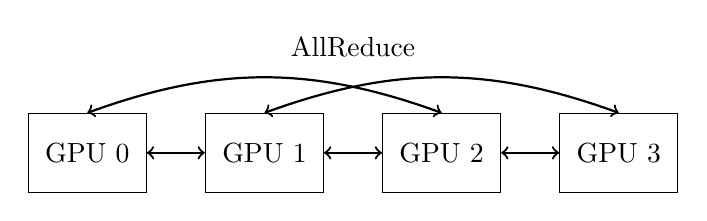
\begin{tikzpicture}[scale=0.9]
        % GPUs
        \foreach \i in {0, 1, 2, 3} {
            \node[draw, rectangle, minimum width=1.5cm, minimum height=1cm] (gpu\i) at (\i*2.5, 0) {GPU \i};
        }
        % AllReduce
        \draw[<->, thick] (gpu0) -- (gpu1);
        \draw[<->, thick] (gpu1) -- (gpu2);
        \draw[<->, thick] (gpu2) -- (gpu3);
        \draw[<->, thick] (gpu0.north) to[bend left=20] (gpu2.north);
        \draw[<->, thick] (gpu1.north) to[bend left=20] (gpu3.north);
        \node at (3.75, 1.5) {AllReduce};
    \end{tikzpicture}
    \caption{AllReduce: each GPU sends its gradients and receives the average.}
    \label{fig:allreduce}
\end{figure}

\newthought{Why it works:}
\begin{equation}
    \mathbb{E}[\bar{g}] = \mathbb{E}\left[\frac{1}{K}\sum_k g_k\right] = \frac{1}{K}\sum_k \mathbb{E}[g_k] = \mathbb{E}[g] = \nabla L(\theta)
\end{equation}

The averaged gradient is still an unbiased estimate of the true gradient!

\marginnote{\newthought{Effective batch size:} With $K$ GPUs and local batch size $b$, the effective batch size is $Kb$. This affects learning rate selection.}


\subsection{Scaling Laws}
\index{scaling laws}

\newthought{Ideal scaling:} $K$ GPUs $\Rightarrow$ $K\times$ speedup.

\newthought{Reality:} Communication overhead limits scaling.

\begin{equation}
    \text{Speedup} = \frac{K}{1 + \frac{t_{\text{comm}}}{t_{\text{compute}}}}
\end{equation}

\newthought{Linear scaling rule:} When batch size increases by $K\times$, increase learning rate by $K\times$ (up to a point).

This keeps the variance of the gradient estimate roughly constant.




\newpage
\section{Model Parallelism}
\index{model parallelism}

\newthought{When the model doesn't fit} on one GPU.

GPT-3 (175B parameters) in FP16: $175 \times 10^9 \times 2 = 350$ GB.
Single GPU: 40--80 GB.
\textbf{Solution:} Split the model across GPUs.

\subsection{Pipeline Parallelism}
\index{pipeline parallelism}

\newthought{Split by layers:} GPU 0 has layers 1--10, GPU 1 has layers 11--20, etc.

\begin{figure}[h]
    \centering
    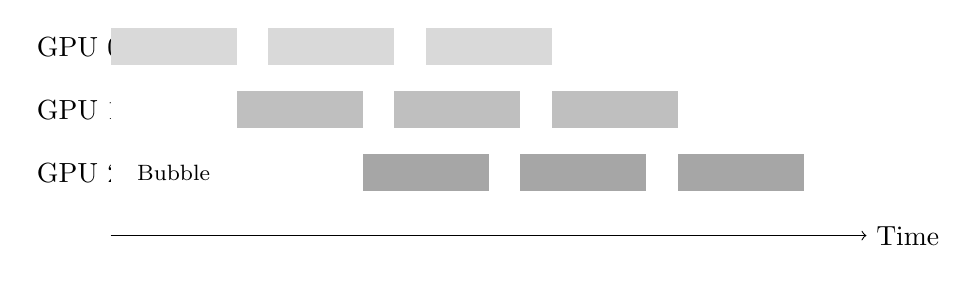
\begin{tikzpicture}[scale=0.8]
        % Timeline
        \draw[->] (0, 0) -- (12, 0) node[right] {Time};
        % GPU labels
        \node at (-0.5, 3) {GPU 0};
        \node at (-0.5, 2) {GPU 1};
        \node at (-0.5, 1) {GPU 2};

        % Micro-batches for GPU 0
        \fill[gray!30] (0, 2.7) rectangle (2, 3.3);
        \fill[gray!30] (2.5, 2.7) rectangle (4.5, 3.3);
        \fill[gray!30] (5, 2.7) rectangle (7, 3.3);

        % Micro-batches for GPU 1
        \fill[gray!50] (2, 1.7) rectangle (4, 2.3);
        \fill[gray!50] (4.5, 1.7) rectangle (6.5, 2.3);
        \fill[gray!50] (7, 1.7) rectangle (9, 2.3);

        % Micro-batches for GPU 2
        \fill[gray!70] (4, 0.7) rectangle (6, 1.3);
        \fill[gray!70] (6.5, 0.7) rectangle (8.5, 1.3);
        \fill[gray!70] (9, 0.7) rectangle (11, 1.3);

        % Bubble
        \fill[white] (0, 1.7) rectangle (2, 2.3);
        \fill[white] (0, 0.7) rectangle (4, 1.3);
        \node at (1, 1) {\footnotesize Bubble};
    \end{tikzpicture}
    \caption{Pipeline parallelism: micro-batches flow through stages. ``Bubbles'' represent idle time.}
    \label{fig:pipeline}
\end{figure}

\newthought{Problem:} Pipeline bubbles---GPUs wait for data from previous stages.

\newthought{Solution:} Micro-batching---process multiple small batches concurrently.


\subsection{Tensor Parallelism}
\index{tensor parallelism}

\newthought{Split individual operations.} For matrix multiply $Y = XW$:
\begin{itemize}
    \item Split $W$ column-wise across GPUs
    \item Each GPU computes part of $Y$
    \item Communicate to assemble full result
\end{itemize}

Used in Megatron-LM for transformer layers.




\newpage
\section{Modern Frameworks}
\index{DeepSpeed}
\index{FSDP}

\newthought{Training billion-parameter models} requires sophisticated frameworks.

\subsection{ZeRO (Zero Redundancy Optimizer)}
\index{ZeRO}

\newthought{Observation:} In data parallelism, each GPU stores a full copy of:
\begin{itemize}
    \item Model parameters
    \item Gradients
    \item Optimizer states (momentum, variance in Adam)
\end{itemize}

This is redundant!

\newthought{ZeRO stages:}
\begin{itemize}
    \item \textbf{Stage 1:} Partition optimizer states
    \item \textbf{Stage 2:} Partition gradients
    \item \textbf{Stage 3:} Partition parameters (FSDP)
\end{itemize}

\marginnote{\newthought{Memory savings:}
\begin{itemize}
    \item Standard: $16 \times$ parameters
    \item ZeRO-3: $\frac{16}{K} \times$ parameters
\end{itemize}
With 64 GPUs: 64$\times$ memory reduction!}


\subsection{Fully Sharded Data Parallel (FSDP)}
\index{FSDP}

PyTorch's implementation of ZeRO-3:
\begin{itemize}
    \item Parameters sharded across GPUs
    \item Gathered just-in-time for computation
    \item Gradients reduced and sharded
\end{itemize}

Enables training models that don't fit on a single GPU, with near-linear scaling.




% ==============================================================================================
% COURSE SYNTHESIS

\newpage
\section{Course Synthesis}
\index{course synthesis}

\newthought{Every large model} uses all the numerical methods we've learned:

\begin{table*}[ht]
\centering
\begin{tabular}{p{0.22\textwidth}p{0.56\textwidth}}
\toprule
\textbf{Concept} & \textbf{Application in LLM Training} \\
\midrule
Discretization & Tokenization, finite parameters, batching \\
Floating-point & Mixed precision (FP16/BF16/FP32) \\
Error analysis & Convergence monitoring, loss curves \\
Newton methods & Gradient-based optimization \\
Complexity & Algorithm selection, scaling analysis \\
SGD & AdamW optimizer, learning rate schedules \\
Stability & Gradient clipping, careful initialization \\
Integration & Batch averaging as Monte Carlo \\
Interpolation & Function approximation via networks \\
Splines & Smooth activation functions \\
Fourier & Positional encoding in transformers \\
ODEs & ResNets, Neural ODEs, diffusion models \\
\textbf{Parallelism} & Data/model parallel distributed training \\
\bottomrule
\end{tabular}
\vspace{2em}
\caption{Every concept from this course appears in modern LLM training. Numerical methods are the foundation of AI.}
\label{tab:course_synthesis}
\end{table*}

\marginnote{\newthought{The complete picture:} Modern AI is built on numerical methods. Understanding these foundations lets you debug training, optimize performance, and push the boundaries of what's possible.}

\newthought{Numerical thinking:}
\begin{itemize}
    \item What's the error? (conditioning, precision)
    \item Is it stable? (gradient flow, numerical tricks)
    \item Will it converge? (optimization theory)
    \item How fast? (complexity, convergence rates)
    \item How does it scale? (parallelism, distribution)
\end{itemize}

\newthought{You now have the complete numerical foundation of modern AI.}




% ==============================================================================================
% STUDENT ACTIVATION BLOCK

\newpage
\section{Examples \& Exercises}
\index{parallel computing!exercises}

\marginnote{\newthought{Code} can be found at \url{https://github.com/Quillstacks/lecturecode_numericalmethods.git}.}

\newthought{Exercise 1: Scaling calculation.} You have access to 8 GPUs, each with 40 GB memory.
\begin{enumerate}
    \item Can you fit GPT-2 (1.5B params) with data parallelism?
    \item What about GPT-3 (175B params)?
    \item How would you train GPT-3 on this hardware?
\end{enumerate}

\textit{Hints:}
\begin{itemize}
    \item Parameters in FP16: $N \times 2$ bytes
    \item Adam optimizer states: $3 \times$ parameters
    \item Total memory needed: $\sim 16 \times$ parameters
\end{itemize}


\vspace{2em}
\newthought{Exercise 2: AllReduce communication.} With $K$ GPUs and gradient size $G$ bytes:
\begin{enumerate}
    \item How much data does each GPU send in naive AllReduce?
    \item How much with ring AllReduce?
    \item Why is ring AllReduce preferred?
\end{enumerate}


\vspace{2em}
\newthought{Exercise 3: Linear scaling rule.} You're training with batch size 64 and LR 0.01.
\begin{enumerate}
    \item You add 3 more GPUs (4 total). What batch size and LR?
    \item You scale to 64 GPUs. What adjustment?
    \item Why does this rule break down for very large batches?
\end{enumerate}


\vspace{2em}
\newthought{Exercise 4: Course synthesis.} For training a transformer model:
\begin{enumerate}
    \item Which chapter explains positional encoding?
    \item Which chapter explains why we use Adam?
    \item Which chapter explains log-softmax stability?
    \item Which chapter explains why SGD works?
\end{enumerate}




\newpage
\section{Self-Reflection and Recap}
\index{parallel computing!recap}

\newthought{Self-Reflection} Questions to guide your understanding:
\begin{itemize}
    \item Why does larger batch size need larger learning rate?
    \item What's the communication cost of AllReduce with $K$ GPUs?
    \item When should you use model parallelism vs. data parallelism?
    \item Why is memory bandwidth often the bottleneck on GPUs?
    \item How do all the concepts from this course fit together?
\end{itemize}

\newthought{Recap} of Key Concepts:
\begin{itemize}
    \item \textbf{Scale problem:} Modern AI requires massive parallelism.
    \item \textbf{GPU architecture:} Optimized for throughput, not latency.
    \item \textbf{Data parallelism:} Replicate model, split data, average gradients.
    \item \textbf{Model parallelism:} Split model when it doesn't fit on one GPU.
    \item \textbf{ZeRO/FSDP:} Partition optimizer states to reduce memory redundancy.
\end{itemize}


\vspace{2em}
\newthought{Course Complete.}

You now understand the numerical foundations of modern AI:
\begin{itemize}
    \item How computers represent and compute with numbers
    \item How to analyze and ensure correctness of numerical methods
    \item How optimization algorithms find good parameters
    \item How to keep computations numerically stable
    \item How to compute integrals and approximate functions
    \item How to analyze signals and simulate dynamics
    \item How to scale computation to massive problems
\end{itemize}

\marginnote{\newthought{What's next?}
\begin{itemize}
    \item Implement these methods yourself
    \item Debug real training failures
    \item Read papers with numerical understanding
    \item Push the boundaries of AI
\end{itemize}}

These fundamentals underpin everything from training GPT-4 to deploying models on edge devices.
Use them wisely.



%%%%%%%%%%%%%%%%%%%%%%%%%%%%%%%%%%%%%%%%%%%%%%%%%%%%%%%%%%%%%%%%%%%%%%%%%%%%%%
